\documentclass[10pt,letterpaper]{article}
\usepackage[top=1in,bottom=1in,left=1in,right=1in]{geometry}
\usepackage{datetime}
\usepackage{natbib}      % http://merkel.zoneo.net/Latex/natbib.php
\usepackage{palatino}
\usepackage{verbatim}
\usepackage[normalem]{ulem}
\bibpunct{(}{)}{;}{a}{,}{,}

\usepackage{array}

\usepackage{chngpage}
\usepackage{stmaryrd}
\usepackage{amssymb}
\usepackage{amsmath}
\usepackage{graphicx}
\usepackage{lscape}
\usepackage{subfigure}
\usepackage[usenames,dvipsnames]{color}
\definecolor{myblue}{rgb}{0,0.1,0.6}
\definecolor{mygreen}{rgb}{0,0.3,0.1}
\usepackage[colorlinks=true,linkcolor=black,citecolor=mygreen,urlcolor=myblue]{hyperref}

\newcommand{\bocomment}[1]{\textcolor{Bittersweet}{BO says: #1}}

\newcommand{\ignore}[1]{}
\newcommand{\transpose}{^\mathsf{T}}
\newcommand{\inner}[1]{\langle #1 \rangle} 
\newcommand{\smallsec}[1]{\noindent \textbf{#1\ }}
\newcommand{\cmd}[1] {{\color{blue}\texttt{#1}}}

\newcommand{\solution}[1]{{\color{myblue} \emph{[Solution:} 

#1 

\emph{End solution]}}}
\newcommand{\solutionnote}[1]{{\color{myblue} \emph{[Note:}

#1 

\emph{End note]}}}
\newcommand{\points}[1]{{\color{mygreen}\emph{[#1]\ \ }}}

\newcommand{\aone}{\diamondsuit}
\newcommand{\atwo}{\heartsuit}
\newcommand{\bone}{\triangle}
\newcommand{\btwo}{\Box}
\newcommand{\myand}{\ \land\ }
\newcommand{\myor}{\ \lor\ }
\newcommand{\mynot}{\lnot}

\title{
  Mini-project 1 \\
  \Large{COMPSCI 370, Spring 2021, UMass Amherst} \\
  \Large{Instructor: Subhransu Maji} \\
  \Large{TAs: Chenyun Wu, Jong-Chyi Su}
}

\settimeformat{ampmtime}
\date{}
\begin{document}
\maketitle

\renewcommand\thesubsection{\thesection.\alph{subsection}}
\section*{Guidelines}
\paragraph{Submission.} Submit a \emph{single pdf} file via
Gradescope that includes your solutions, figures, and code. The latex
source file for the homework is provided in case you want to modify it
to produce your report. However, you are welcome to use other
typesetting software as long as the final output is a pdf.
For readability you may attach the code printouts at the end of the
solutions within the same pdf.
Similarly figures enable easy comparision of various approaches.
Poorly written or formatted reports will make it harder for us to
evaluate it and may lead to a deduction of credit.


\paragraph{Late policy.}
\begin{itemize}
\item You can use 7 late days, with up to 3 late days per assignment.
\item Once you have used all 7 late days, penalty is 25\% for each additional late day.
\item We will use your latest submission for grading and for calculating your late day usage.
\item There is no bonus if you don't use late days at all.
\end{itemize}


\paragraph{Plagiarism.}
We expect the students not to copy, refer to, or look at the solutions
in preparing their answers. We expect students to want to learn and
not google for answers. See the Universities' guidelines on academic
honesty (\url{https://www.umass.edu/honesty}).
Finally, we also ask you to not post the solutions online as the
problem sets might be used in future.


\paragraph{Collaboration.} The homework must be done individually,
except where otherwise noted in the assignments. 'Individually' means
each student must hand in their own answers, and each student must
write their own code in the programming part of the assignment. It is
acceptable, however, for students to collaborate in figuring out
answers and helping each other solve the problems, for example within
a study group.
We will be assuming that you will be taking the responsibility to make
sure you personally understand the solution to any work arising from
such a collaboration.


\paragraph{Python requirements.}
Our code is tested on Python 3.
The Python code depends on external
packages such as \cmd{scipy}, \cmd{numpy}, and \cmd{scikit-image}.
Take a look at the resources posted on the course page to set up the
appropriate programming environment and tutorial on basic concepts.


\paragraph{Using other programming languages.}
While we have made the starter code available in Python, 
feel free to implement the homework from scratch using your favorite
programming language. For example you are welcome to use Matlab, C, Java,
Octave or Julia, with the caveat that we may be able help you with
debugging.







\newpage
\section{Matrix manipulation [8 points]}
The following tests basic matrix manipulation skills in Python. Follow
the Python and linear algebra tutorial on the course page to refesh your skills.
\begin{enumerate}
\item \points{1 point} Create a $m \times n$ array of all zeros (double precision)
\item \points{1 point} Create a $m \times n$ array with each entry
  uniformly distributed in the interval $[0, 1]$, i.e. each value
  between $0$ and $1$ is equally likely (double precision)
\item \points{2 points} You can represent vectors as matrices of size
  $n \times 1$. Given a vector represented as a variable $v$, write
  down the code to compute its length (or norm). You may find the functions \cmd{sum()} and element-wise
  squaring \cmd{.\textasciicircum 2} useful to do this without for loops.
\item  Given $u$ and $v$ representing arrays of size $n \times 1$,
  write down code to compute their
\begin{enumerate}
\item \points{1 point} dot product
\item \points{1 point} angle
\item \points{1 point} Euclidean distance
\end{enumerate}
Implement these using standard primitives in numpy (e.g., loops and basic
math operations) and not inbuilt functions in \cmd{np.linalg} for example.
\item \points{1 point} Given an array $a \in \mathbb{R}^{m\times n}$
  write code to reshape it to a vector of size $nm \times 1$.
\end{enumerate}


\section{Image formation [15 points]}
Assume you have a pinhole camera made out of a shoebox of size 15cm x 15cm x
30cm.
It has a hole on the 15cm x 15cm side and an image is formed on the
opposite side.
Assume that an 1 meter tall object is at a distance of 15 meters from
the pinhole along the projection axis.
\begin{enumerate}
\item \points{4 points} Draw a picture illustrating the object and the image formed in the pinhole camera. Clearly show the marked dimensions.
\item \points{2 points} What is the size of the object in the pinhole image?
\item \points{2 points} At what distance does the image of the object \emph{entirely} occupy the projection screen (\emph{note:} the size of the screen is 15cm x 15 cm).
\item \points{2 points} Suppose it took 10 milliseconds to capture an
  image using a pinhole camera with aperture radius of 1mm. How long
  would it take to capture the same amount of light using a camera
  with a lens of radius 10mm?
\end{enumerate}

\noindent
\points{5 points} Show that any two lines that are parallel to each
  other in 3D have the same vanishing point. Your proof can be a
  geometric or algebraic one.

\section{Light [30 points]}
\subsection{Linearity [5 points]}
Alice has a chandelier with 5 light
bulbs sockets. Currently, she has 5 100-watt incandescent bulbs in the sockets.
Each incandescent bulb is characterized by a spectrum $S_{\text{INC}}(\lambda)$, for integer $\lambda$
from 380 to 779, which gives the fraction of the total power output for each
interval with wavelengths between $\lambda$ and $\lambda + 1$ nanometers. For example, if
$S_{\text{INC}}(523) = 0.002$, then it means that the incandescent bulb outputs $0.002 \times
100 = .2$ watts in the range of $523$ -- $524$ nanometer wavelengths.
Eventually, she wants to replace the incandescent bulbs with fancy new
light emitting diode (LED) bulbs (also 100-watt bulbs) that have a different
spectrum $S_{\text{LED}}(\lambda)$, but right now, she only has 3 of these. She replaces 3 of the 5
incandescent bulbs with the LED bulbs. Give a formula for the chandelier’s new
spectrum $S_{\text{TOTAL}}$ in terms of the components of $S_{\text{INC}}$ and $S_{\text{LED}}$. The new spectrum
should give the fraction of the total power at each 1 nanometer portion of the
visible spectrum.


\subsection{Tristimulus theory [25 points]} Let $F_1$, $F_2$, and $F_3$ below
represent the power spectra of 3 different colored flashlights, where each of the 10 values is the fraction of power produced in a 40nm range from 380nm to 780nm. (Note: some of the power will be in the non-visible spectrum).\\

\begin{tabular}{c}
$F_1$ = [0.00, 0.00, 0.00, 0.00, 0.01, 0.02, 0.07, 0.29, 0.35, 0.12];\\
$F_2$ = [0.00, 0.01, 0.02, 0.06, 0.20, 0.31, 0.20, 0.16, 0.04, 0.00];\\
$F_3$ = [0.03, 0.15, 0.25, 0.27, 0.12, 0.02, 0.01, 0.01, 0.00, 0.00];\\
\end{tabular} \\

For example, flashlight F1 produces 12 percent of its power in the range 740-780nm. Figure~\ref{fig:spectra} shows the spectra of the three flashlights.\\

\begin{figure}[h]
\centering
\includegraphics[width=0.8\linewidth]{flashlight-spectrum.pdf}
\caption{\textbf{Three flashlight spectra.} This image shows the three spectra of $F_1$, $F_2$, and $F_3$.}
\label{fig:spectra}
\end{figure}

Let $S_r(\lambda)$, $S_g(\lambda)$, and $S_b(\lambda)$ represent the relative absorption spectra of the cone cells in your eye. This means that, of the power absorbed by a given type of cone cell, the fraction absorbed in a given range is given by these numbers.\\

\begin{tabular}{c}
$S_r(\lambda)$ = [0.16, 0.26, 0.28, 0.15, 0.10, 0.03, 0.02, 0.00, 0.00, 0.00]; \\
$S_g(\lambda)$ = [0.00, 0.03, 0.06, 0.20, 0.31, 0.21, 0.15, 0.03, 0.01, 0.00];\\
$S_b(\lambda)$ = [0.00, 0.00, 0.00, 0.00, 0.01, 0.04, 0.08, 0.23, 0.35, 0.29];
\end{tabular}\\

When a flashlight is 5 meters from a white screen, assume that it stimulates
a cone cell response (relative to the maximum possible response from that cone)
given by: \\
\begin{equation*}
R^f_c = \sum_{i=1}^{10} F_f (i) \times S_c(i).
\end{equation*}

Here $F_f$ is flashlight $f$, $S_c$ is the absorption spectrum for cones of type $c$, and $R^f_c$ is the response for cone cell type $c$ and flashlight $f$. For example, from 5 meters away, the third flashlight $F_3$ generate a response from the green cone cells of\\
\begin{eqnarray*}
R^3_g &=& \sum_{i=1}^{10} F_3 (i) \times S_g(i) \\
&=& 0.03\times0.00 + 0.15\times0.03 + 0.25\times0.06 + 0.27\times0.20 + 0.12\times0.31 + \\ 
&~& 0.02\times0.21 + 0.01\times0.15 + 0.01\times0.03 + 0.00\times0.01 + 0.00\times0.00 \\
&=& 0.1167\\
\end{eqnarray*}

Consider the response of all 3 cone cell types at once to a given flashlight $f$
at a fixed distance from the white screen. We will call this variable $R^f$, and it will be a vector of 3 values:
\[
	R^f = \left[ \begin{array}{c}
				R^f_r \\
				R^f_g \\				
				R^f_b \end{array} \right]
\]

Of course, the “color” that you see for a particular flashlight will be related
to the cone cell responses $R^f$ produced by that flashlight. Due to the linearity
of light and the approximate linearity of cone cell responses, you can model the
responses of the cone cells to two flashlights, say 1 and 3, as

\[
	R^1 + R^3 = \left[ \begin{array}{c}
				R^1_r + R^3_r\\
				R^1_g + R^3_g\\				
				R^1_b + R^3_b\end{array} \right]
\]

\begin{enumerate}
\item \textbf{(10 points)} Let the matrix R be defined to be 
\[
	R = \left[ \begin{array}{ccc}
				R^1_r &  R^2_r & R^3_r\\
				R^1_g &  R^2_g & R^3_g\\
				R^1_b &  R^2_b & R^3_b\end{array} \right]
\]
Write a Python function to compute the matrix $R$ given $F_1$, $F_2$,
$F_3$, $S_r$, $S_g$, and $S_b$. Give the value of the matrix $R$.


\item \textbf{(15 points)} If we had a way to make each flashlight brighter or dimmer, then we could
create novel color combinations. In particular, if we let $b_1$ be the brightness
multiplier for flashlight 1, $b_2$ the brightness multiplier for flashlight 2, and $b_3$ the brightness multiplier for flashlight 3, then we can create arbitrary linear
combinations of the 3 flashlights as
\[
	b_1R^1 + b_2R^2 + b_3R^3 = \left[ \begin{array}{c}
				b_1R^1_r + b_2R^2_r + b_3R^3_r\\
				b_1R^1_g + b_2R^2_g + b_3R^3_g\\				
				b_1R^1_b + b_2R^2_b + b_3R^3_b\end{array} \right]
\]

Now suppose you want to create a combination of lights that results in a
particular perceived color. For example, the color turquoise is perceived when
the RGB cone cells have a response of
\[
C_{\text{turquoise}} = \left[ \begin{array}{c} 0.2509 \\ 0.8784 \\ 0.8156 \end{array} \right]
\]

We need to solve the following set of equations
\begin{eqnarray*}
b_1R^1_r + b_2R^2_r + b_3R^3_r = C_r\\
b_1R^1_g + b_2R^2_g + b_3R^3_g = C_g \\
b_1R^1_b + b_2R^2_b + b_3R^3_b = C_b \\
\end{eqnarray*}
This can be written in matrix form as
\[ Rb = C, \]

where $R$ is the matrix defined previously, $b$ is a vector of 3
multiplier values, and $C$ is the 3 color components for the desired
color. Fortunately, this is extremely easy to solve! By multiplying
both sides by the matrix inverse of $R$, we obtain
\[ R^{-1}Rb = R^{-1}C, \]
and then simplifying,
\[ b = R^{-1}C. \]
In Python, you can use the function \cmd{np.linalg.inv()}.

Write a Python function, which, given the matrix $R$ and a
set of desired color responses in the form of a vector $C$ calculates
the proper brightness multiplier weights $b$ and returns them as a
single vector of 3 values. Using this code compute the multiplier
weights for each flashlight so that you  obtain:

Turquoise: 
\[
C_{\text{turquoise}} = \left[ \begin{array}{c} 0.2509 \\ 0.8784 \\ 0.8156 \end{array} \right]
\]\\

$b_1$: \underline{\hspace{3cm}}, $b_2$: \underline{\hspace{3cm}}, $b_3$:\underline{\hspace{3cm}}

\vspace{0.5in}
Goldenrod (a slightly brownish yellow): 
\[
C_{\text{goldenrod}} = \left[ \begin{array}{c} 0.8549 \\ 0.6470 \\ 0.1254 \end{array} \right]
\]\\

$b_1$: \underline{\hspace{3cm}}, $b_2$: \underline{\hspace{3cm}}, $b_3$:\underline{\hspace{3cm}}

\end{enumerate}


\section{White balance [20 points]}
White balance is the process of adjusting color casts caused by
illumination mismatches.
Our eyes are very good at removing the effect of
illumination to judge the true color of an object, a phenomenon we
described as \emph{color constancy}.
One way to model the effect of a light on a
surface is to assume that the reflected color $I = (i_r,i_g,i_b)$
arises due to light of color $L= (l_r,l_g,l_b)$ interacting with paint
of color $C = (c_r,c_g,c_b)$ satisfying

	$L \times C = I$, i.e. 
	\[ (l_r \times c_r,l_g \times c_g ,\l_b \times c_b) = (i_r,i_g,i_b)
	\]
Assume $(l_r, l_g, l_b)$ is the fractional power of the light in each
of the color channels.
Then, given the light $L$ at a given pixel we
can obtain its true color by dividing the measured intensity with the
light
\[
	c_r = \frac{i_r}{l_r}; 
	c_g = \frac{i_g}{l_g}; 
	c_b = \frac{i_b}{l_b}; 
\]

Unfortunately, computing $L$ and $C$ given $I$ is an ill-posed
problem.
For example, a red pixel of value $I=(255,0,0)$ could be due to a white light
$L=(1,1,1)$ illuminating a red object $C=(255,0,0)$, or red light
$L=(1,0,0)$ illuminating a white object $C=(255,255,255)$, since both these
satisfy $L\times C = I$.

Prior knowledge about the world can help us resolve this ambiguity.
One such prior is the ``gray world'' assumption.
It states the average pixel color under white or neural color light is
gray (recall that any color $(r,g,b)$ where $r=g=b$ is gray.)
For the purposes of this homework we will assume that the average is
$(128,128,128)$ assuming that the color values are between 0 and 255.


\begin{itemize}
\item \textbf{(5 points)} Assuming that the light is uniform across
  all pixels.Show that under the gray world assumption the light $L$ is given by
\[
	L = \left(\frac{r_{ave}}{128}, \frac{g_{ave}}{128}, \frac{b_{ave}}{128}\right),
\]

where, $r_{ave}, g_{ave}, b_{ave}$ are the average of the red, green,
and blue channels of the image.
Thus one can obtain the true color of a pixel as:
\[
	c_r = i_r \times \frac{128}{r_{ave}}; 
	c_g = i_g \times \frac{128}{g_{ave}}; 
	c_b = i_b \times \frac{128}{b_{ave}}; 
\]

\item \textbf{(15 points)} Implement a function $\cmd{[L, C] =
  grayworld(I)}$ that takes an image $\cmd{I}$ and returns the light
  $L$ and color image $C$ using the above calculations. Run your code
  on the image as shown in Figure~\ref{fig:color}, which is $\cmd{wb\_sardmen-incorrect.jpg}$ included in the \cmd{data} directory.
  
Write down the value of $L$ as shown below, include the code for the function and a picture of the
color corrected image $C$ in your solution.

\textbf{Light}~~ $l_r$: \underline{\hspace{2cm}}, $l_g$: \underline{\hspace{3cm}}, $l_b$:\underline{\hspace{3cm}}


Note that the color corrected image will need to be scaled back to the
range of [0,255] or [0,1] to display properly. A simple way of doing
this is to divide all the values by the maximum pixel value across all
channels and scale it back to the appropriate range.
Alternatively you can use \cmd{plt.imshow(C); plt.show()} in Python
with the appropriate arguments.
Also note that if your image is loaded in a floating point format with
intensities between 0 and 1, a white pixel has value $(1.0, 1.0, 1.0)$
and the average can be assumed to be $(0.5, 0.5, 0.5)$.

\end{itemize}

\begin{figure}[h]
\centering
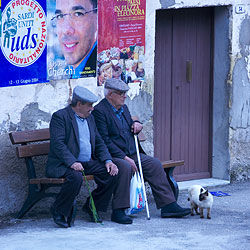
\includegraphics[scale=1]{../data/wb_sardmen-incorrect.jpg}
\caption{Image with a color cast. Source: \url{https://www.cambridgeincolour.com/tutorials/white-balance.htm}}
\label{fig:color}
\end{figure}
\end{document}
